\documentclass[12pt]{standalone}

\usepackage[rgb]{xcolor}
\usepackage{tikz}
\usetikzlibrary{decorations.markings}
\usetikzlibrary{math}

\definecolor{quarkred}{HTML}{ef8a62}
\definecolor{quarkblue}{HTML}{67a9cf}
\definecolor{bg-color}{HTML}{d9d9d9}

\begin{document}
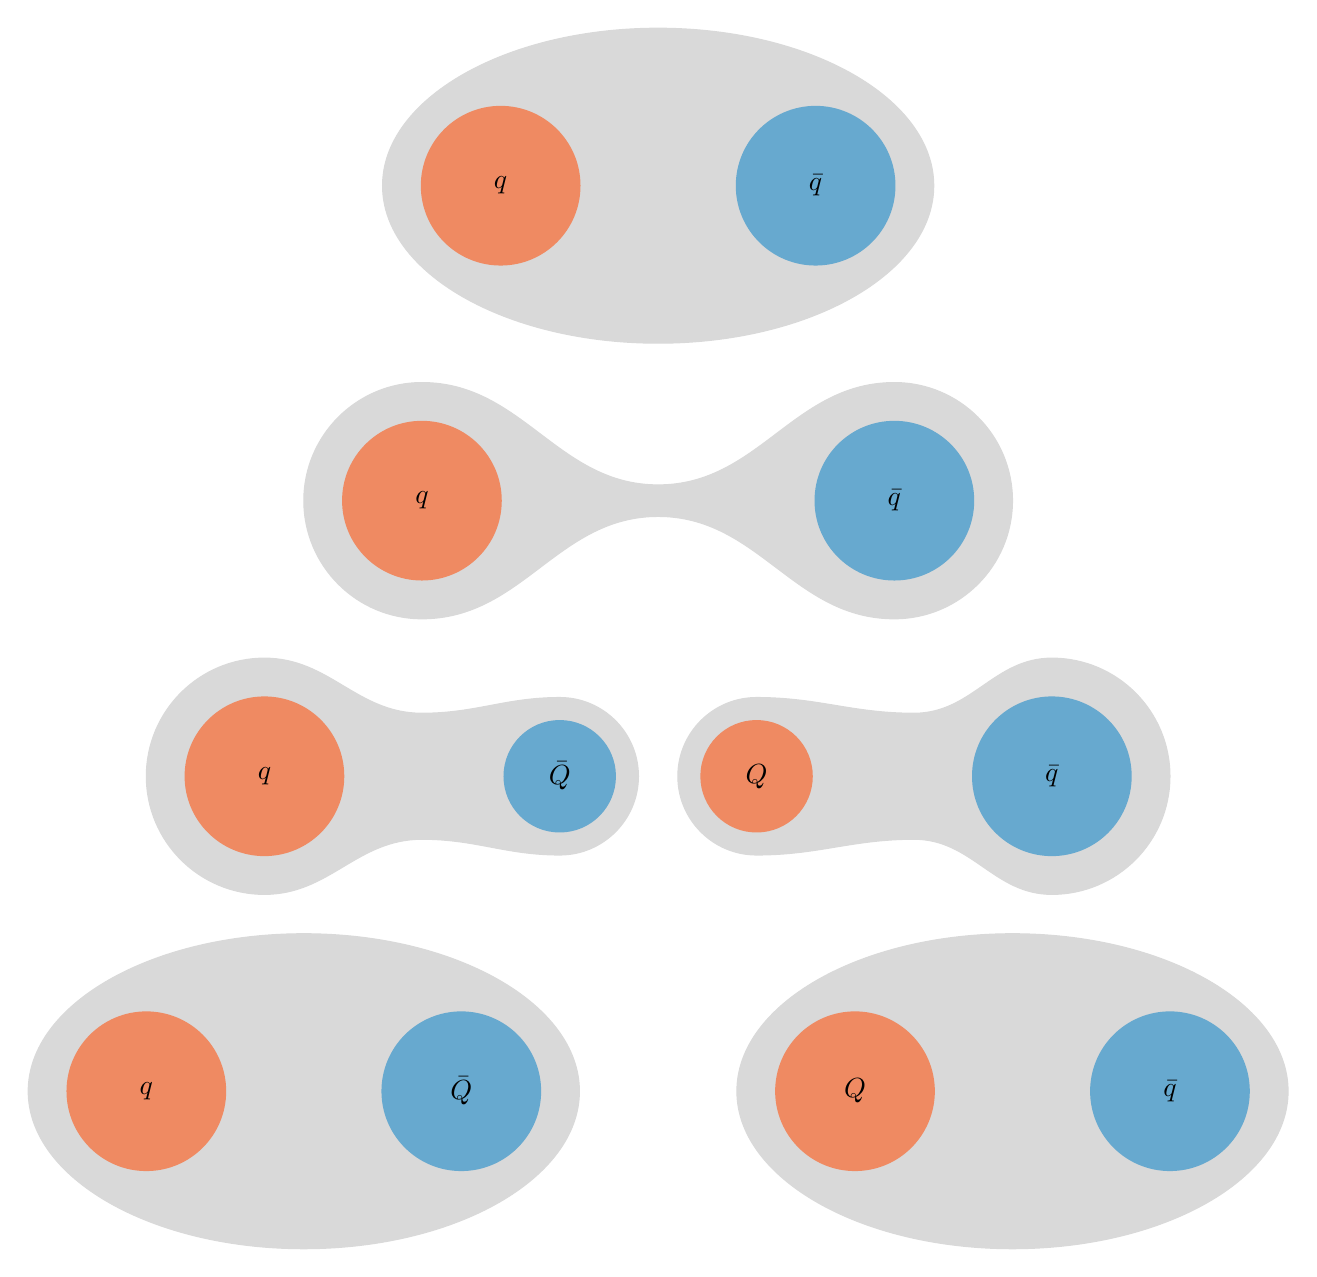
\begin{tikzpicture}

% Position settings
\tikzmath{
    % Top coordinates
    \xmesontop = 2;
    \ymesontop = 4;
    % Middle coordinates
    \ymesonmiddle = 0;
    \xmesonmiddle = 3;
    % Lower coordinates
    \ymesonlower = -3.5;
    \xmesonlower = 5;
    \xmesonlowerRshift = 6.25;
    % Bottom coordinates
    \ymesonbottom = -7.5;
    \xmesonbottom = 4.5;
    \xmesonbotttomRshift = 5;
}

% Draws first meson row
\draw[bg-color,fill] (0,\ymesontop) ellipse (3.5 and 2.0);
\draw[quarkred,thick,fill] (-\xmesontop,\ymesontop) circle[radius=1];
\draw[quarkblue,thick,fill] (+\xmesontop,\ymesontop) circle[radius=1];
\draw[black] (-\xmesontop,\ymesontop) node {$q$};
\draw[black] (+\xmesontop,\ymesontop) node {$\bar{q}$};

% Draws second meson row
\coordinate (A1) at (-\xmesonmiddle,1.5+\ymesonmiddle);
\coordinate (B1) at (0,-0.2+\ymesonmiddle);
\coordinate (C1) at (\xmesonmiddle,-1.5+\ymesonmiddle);
\coordinate (D1) at (\xmesonmiddle,1.5+\ymesonmiddle);
\coordinate (E1) at (0,0.2+\ymesonmiddle);
\coordinate (F1) at (-\xmesonmiddle,1.5+\ymesonmiddle);
\path[
    draw,
    bg-color,
    fill,
    ]
    (A1) arc (90:270:1.5) to[out=0, in=180] (B1) to[out=0, in=180] (C1) arc (270:450:1.5) to[out=180, in=0] (D1) to[out=180, in=0] (E1) to[out=180, in=0] (F1);
\draw[quarkred,thick,fill] (-\xmesonmiddle,\ymesonmiddle) circle[radius=1];
\draw[quarkblue,thick,fill] (+\xmesonmiddle,\ymesonmiddle) circle[radius=1];
\draw[black] (-\xmesonmiddle,\ymesonmiddle) node {$q$};
\draw[black] (+\xmesonmiddle,\ymesonmiddle) node {$\bar{q}$};

% \draw[black, very thick, <->] (-0.5*\xmesonmiddle, 1.5) -- (0.5*\xmesonmiddle, 1.5);

% Draws third meson row. Two new quarks have just formed.
% Left meson
\coordinate (A2L) at (-\xmesonlower,1.5+\ymesonlower);
\coordinate (B2L) at (-3.0,-0.8+\ymesonlower);
\coordinate (C2L) at (-0.25*\xmesonlower,-1.0+\ymesonlower);
\coordinate (D2L) at (-0.25*\xmesonlower,1.0+\ymesonlower);
\coordinate (E2L) at (-3.0,0.8+\ymesonlower);
\coordinate (F2L) at (-\xmesonlower,1.5+\ymesonlower);
\path[
    draw,
    bg-color,
    fill,
    ]
    (A2L) arc (90:270:1.5) to[out=0, in=180] (B2L) to[out=0, in=180] (C2L) arc (270:450:1.0) to[out=180, in=0] (D2L) to[out=180, in=0] (E2L) to[out=180, in=0] (F2L);
\draw[quarkred,thick,fill] (-\xmesonlower,\ymesonlower) circle[radius=1];
\draw[quarkblue,thick,fill] (-0.25*\xmesonlower,\ymesonlower) circle[radius=0.7];
\draw[black] (-\xmesonlower,\ymesonlower) node {$q$};
\draw[black] (-0.25*\xmesonlower,\ymesonlower) node {$\bar{Q}$};

% Right meson
\coordinate (A2R) at (-\xmesonlower+\xmesonlowerRshift,1.0+\ymesonlower);
\coordinate (B2R) at (-3.0+\xmesonlowerRshift,-0.8+\ymesonlower);
\coordinate (C2R) at (-0.25*\xmesonlower+\xmesonlowerRshift,-1.5+\ymesonlower);
\coordinate (D2R) at (-0.25*\xmesonlower+\xmesonlowerRshift,1.5+\ymesonlower);
\coordinate (E2R) at (-3.0+\xmesonlowerRshift,0.8+\ymesonlower);
\coordinate (F2R) at (-\xmesonlower+\xmesonlowerRshift,1.0+\ymesonlower);
\path[
    draw,
    bg-color,
    fill,
    ]
    (A2R) arc (90:270:1.0) to[out=0, in=180] (B2R) to[out=0, in=180] (C2R) arc (270:450:1.5) to[out=180, in=0] (D2R) to[out=180, in=0] (E2R) to[out=180, in=0] (F2R);
\draw[quarkred,thick,fill] (0.25*\xmesonlower,\ymesonlower) circle[radius=0.7];
\draw[quarkblue,thick,fill] (\xmesonlower,\ymesonlower) circle[radius=1.0];
\draw[black] (0.25*\xmesonlower,\ymesonlower) node {$Q$};
\draw[black] (\xmesonlower,\ymesonlower) node {$\bar{q}$};


% Draws fourth meson row. Two new stable mesons have formed.
% Left meson
\draw[bg-color,fill] (-\xmesonbottom,\ymesonbottom) ellipse (3.5 and 2.0);
\draw[quarkred,thick,fill] (-\xmesonbottom-\xmesontop,\ymesonbottom) circle[radius=1];
\draw[quarkblue,thick,fill] (-\xmesonbottom+\xmesontop,\ymesonbottom) circle[radius=1];
\draw[black] (-\xmesonbottom-\xmesontop,\ymesonbottom) node {$q$};
\draw[black] (-\xmesonbottom+\xmesontop,\ymesonbottom) node {$\bar{Q}$};

% Right meson
\draw[bg-color,fill] (+\xmesonbottom,\ymesonbottom) ellipse (3.5 and 2.0);
\draw[quarkred,thick,fill] (+\xmesonbottom-\xmesontop,\ymesonbottom) circle[radius=1];
\draw[quarkblue,thick,fill] (+\xmesonbottom+\xmesontop,\ymesonbottom) circle[radius=1];
\draw[black] (+\xmesonbottom-\xmesontop,\ymesonbottom) node {$Q$};
\draw[black] (+\xmesonbottom+\xmesontop,\ymesonbottom) node {$\bar{q}$};


% \path[draw] (0,4) to (0,-4);
% \path[draw] (-\xmesonlower,4) to (-\xmesonlower,-4);
% \path[draw] (\xmesonlower,4) to (\xmesonlower,-4);
% \path[draw] (-\xmesonlower,-3) to (\xmesonlower,-3);
% \path[draw] (-\xmesonlower,-4) to (\xmesonlower,-4);
% \path[draw] (-\xmesonlower,-5) to (\xmesonlower,-5);

\end{tikzpicture}
\end{document}